\documentclass{standalone}
\usepackage{tikz}
\usetikzlibrary{patterns, positioning}

\begin{document}
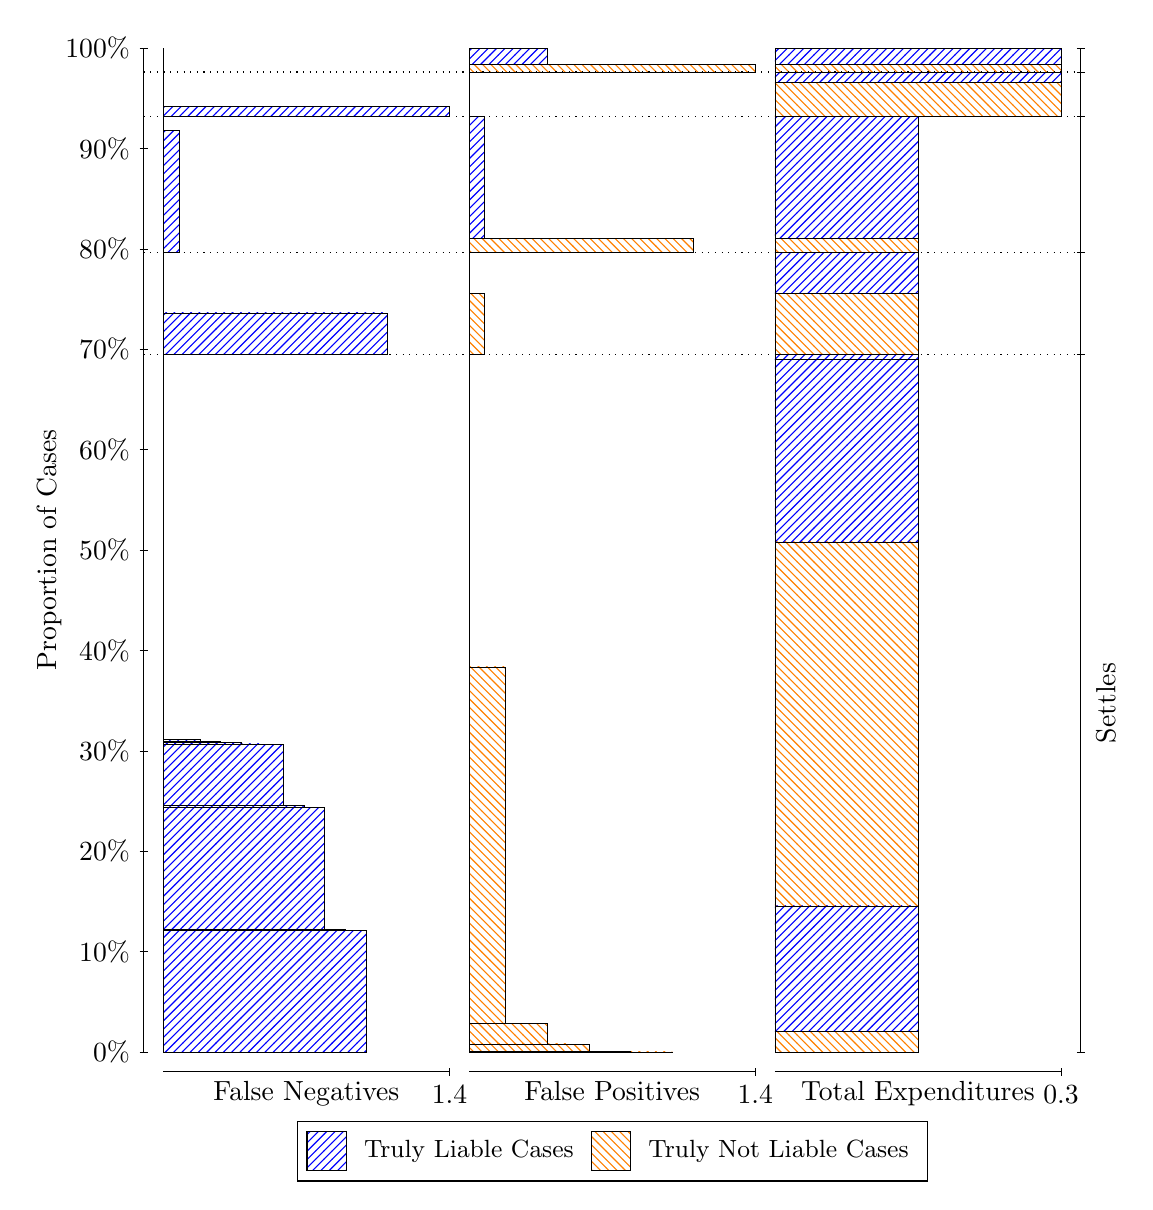
\begin{tikzpicture}
\draw[black, very thin] (1.5,1.75) -- (1.5,14.5);
\node[rotate=90, anchor=center] at (0.3, 8.125) {Proportion of Cases};
\draw[black, very thin] (1.45,1.75) -- (1.55,1.75);
\node[anchor=east] at (1.45, 1.75) {0\%};
\draw[black, very thin] (1.45,3.025) -- (1.55,3.025);
\node[anchor=east] at (1.45, 3.025) {10\%};
\draw[black, very thin] (1.45,4.3) -- (1.55,4.3);
\node[anchor=east] at (1.45, 4.3) {20\%};
\draw[black, very thin] (1.45,5.575) -- (1.55,5.575);
\node[anchor=east] at (1.45, 5.575) {30\%};
\draw[black, very thin] (1.45,6.85) -- (1.55,6.85);
\node[anchor=east] at (1.45, 6.85) {40\%};
\draw[black, very thin] (1.45,8.125) -- (1.55,8.125);
\node[anchor=east] at (1.45, 8.125) {50\%};
\draw[black, very thin] (1.45,9.4) -- (1.55,9.4);
\node[anchor=east] at (1.45, 9.4) {60\%};
\draw[black, very thin] (1.45,10.675) -- (1.55,10.675);
\node[anchor=east] at (1.45, 10.675) {70\%};
\draw[black, very thin] (1.45,11.95) -- (1.55,11.95);
\node[anchor=east] at (1.45, 11.95) {80\%};
\draw[black, very thin] (1.45,13.225) -- (1.55,13.225);
\node[anchor=east] at (1.45, 13.225) {90\%};
\draw[black, very thin] (1.45,14.5) -- (1.55,14.5);
\node[anchor=east] at (1.45, 14.5) {100\%};

\draw[black, very thin] (13.4,1.75) -- (13.4,14.5);
\draw[black, very thin] (13.35,1.75) -- (13.45,1.75);
\node[anchor=west] at (13.35, 1.75) {};
\draw[black, very thin] (13.35,10.611) -- (13.45,10.611);
\node[anchor=west] at (13.35, 10.611) {};
\draw[black, very thin] (13.35,11.907) -- (13.45,11.907);
\node[anchor=west] at (13.35, 11.907) {};
\draw[black, very thin] (13.35,13.631) -- (13.45,13.631);
\node[anchor=west] at (13.35, 13.631) {};
\draw[black, very thin] (13.35,14.195) -- (13.45,14.195);
\node[anchor=west] at (13.35, 14.195) {};
\draw[black, very thin] (13.35,14.5) -- (13.45,14.5);
\node[anchor=west] at (13.35, 14.5) {};

\draw[black, very thin, pattern color=blue, pattern=north east lines] (1.75,1.75) rectangle (4.3264,3.2925);
\draw[black, very thin, pattern color=blue, pattern=north east lines] (1.75,3.2925) rectangle (4.0621,3.3055);
\draw[black, very thin, pattern color=blue, pattern=north east lines] (1.75,3.3055) rectangle (3.7979,4.8567);
\draw[black, very thin, pattern color=blue, pattern=north east lines] (1.75,4.8567) rectangle (3.5336,4.8851);
\draw[black, very thin, pattern color=blue, pattern=north east lines] (1.75,4.8851) rectangle (3.2694,5.6551);
\draw[black, very thin, pattern color=blue, pattern=north east lines] (1.75,5.6551) rectangle (3.0052,5.6628);
\draw[black, very thin, pattern color=blue, pattern=north east lines] (1.75,5.6628) rectangle (2.7409,5.6851);
\draw[black, very thin, pattern color=blue, pattern=north east lines] (1.75,5.6851) rectangle (2.4767,5.6914);
\draw[black, very thin, pattern color=blue, pattern=north east lines] (1.75,5.6914) rectangle (2.2124,5.7211);
\draw[black, very thin, pattern color=orange, pattern=north west lines] (1.75,5.7211) rectangle (1.75,10.611);
\draw[black, very thin, pattern color=blue, pattern=north east lines] (1.75,10.611) rectangle (4.5906,11.137);
\draw[black, very thin, pattern color=orange, pattern=north west lines] (1.75,11.137) rectangle (1.75,11.907);
\draw[black, very thin, pattern color=blue, pattern=north east lines] (1.75,11.907) rectangle (1.9482,13.454);
\draw[black, very thin, pattern color=orange, pattern=north west lines] (1.75,13.454) rectangle (1.75,13.631);
\draw[black, very thin, pattern color=blue, pattern=north east lines] (1.75,13.631) rectangle (5.3833,13.758);
\draw[black, very thin, pattern color=orange, pattern=north west lines] (1.75,13.758) rectangle (1.75,14.195);
\draw[black, very thin, pattern color=orange, pattern=north west lines] (1.75,14.195) rectangle (1.75,14.296);
\draw[black, very thin, pattern color=blue, pattern=north east lines] (1.75,14.296) rectangle (1.75,14.5);
\draw[black, very thin, pattern color=orange, pattern=north west lines] (5.6333,1.75) rectangle (8.2097,1.7517);
\draw[black, very thin, pattern color=orange, pattern=north west lines] (5.6333,1.7517) rectangle (7.9455,1.7521);
\draw[black, very thin, pattern color=orange, pattern=north west lines] (5.6333,1.7521) rectangle (7.6812,1.7534);
\draw[black, very thin, pattern color=orange, pattern=north west lines] (5.6333,1.7534) rectangle (7.417,1.7539);
\draw[black, very thin, pattern color=orange, pattern=north west lines] (5.6333,1.7539) rectangle (7.1527,1.8504);
\draw[black, very thin, pattern color=orange, pattern=north west lines] (5.6333,1.8504) rectangle (6.8885,1.8523);
\draw[black, very thin, pattern color=orange, pattern=north west lines] (5.6333,1.8523) rectangle (6.8885,1.8533);
\draw[black, very thin, pattern color=orange, pattern=north west lines] (5.6333,1.8533) rectangle (6.6242,2.1114);
\draw[black, very thin, pattern color=orange, pattern=north west lines] (5.6333,2.1114) rectangle (6.36,2.1123);
\draw[black, very thin, pattern color=orange, pattern=north west lines] (5.6333,2.1123) rectangle (6.0958,6.6403);
\draw[black, very thin, pattern color=blue, pattern=north east lines] (5.6333,6.6403) rectangle (5.6333,10.611);
\draw[black, very thin, pattern color=orange, pattern=north west lines] (5.6333,10.611) rectangle (5.8315,11.381);
\draw[black, very thin, pattern color=blue, pattern=north east lines] (5.6333,11.381) rectangle (5.6333,11.907);
\draw[black, very thin, pattern color=orange, pattern=north west lines] (5.6333,11.907) rectangle (8.4739,12.084);
\draw[black, very thin, pattern color=blue, pattern=north east lines] (5.6333,12.084) rectangle (5.8315,13.631);
\draw[black, very thin, pattern color=orange, pattern=north west lines] (5.6333,13.631) rectangle (5.6333,14.068);
\draw[black, very thin, pattern color=blue, pattern=north east lines] (5.6333,14.068) rectangle (5.6333,14.195);
\draw[black, very thin, pattern color=orange, pattern=north west lines] (5.6333,14.195) rectangle (9.2667,14.296);
\draw[black, very thin, pattern color=blue, pattern=north east lines] (5.6333,14.296) rectangle (6.6242,14.5);
\draw[black, very thin, pattern color=orange, pattern=north west lines] (9.5167,1.75) rectangle (11.333,2.0119);
\draw[black, very thin, pattern color=blue, pattern=north east lines] (9.5167,2.0119) rectangle (11.333,3.6045);
\draw[black, very thin, pattern color=orange, pattern=north west lines] (9.5167,3.6045) rectangle (11.333,8.229);
\draw[black, very thin, pattern color=blue, pattern=north east lines] (9.5167,8.229) rectangle (11.333,10.541);
\draw[black, very thin, pattern color=orange, pattern=north west lines] (9.5167,10.541) rectangle (11.333,10.545);
\draw[black, very thin, pattern color=blue, pattern=north east lines] (9.5167,10.545) rectangle (11.333,10.611);
\draw[black, very thin, pattern color=orange, pattern=north west lines] (9.5167,10.611) rectangle (11.333,11.381);
\draw[black, very thin, pattern color=blue, pattern=north east lines] (9.5167,11.381) rectangle (11.333,11.907);
\draw[black, very thin, pattern color=orange, pattern=north west lines] (9.5167,11.907) rectangle (11.333,12.084);
\draw[black, very thin, pattern color=blue, pattern=north east lines] (9.5167,12.084) rectangle (11.333,13.631);
\draw[black, very thin, pattern color=orange, pattern=north west lines] (9.5167,13.631) rectangle (13.15,14.068);
\draw[black, very thin, pattern color=blue, pattern=north east lines] (9.5167,14.068) rectangle (13.15,14.195);
\draw[black, very thin, pattern color=orange, pattern=north west lines] (9.5167,14.195) rectangle (13.15,14.296);
\draw[black, very thin, pattern color=blue, pattern=north east lines] (9.5167,14.296) rectangle (13.15,14.5);
\draw[black, dotted] (1.5,10.611) -- (13.4,10.611);
\draw[black, dotted] (1.5,11.907) -- (13.4,11.907);
\draw[black, dotted] (1.5,13.631) -- (13.4,13.631);
\draw[black, dotted] (1.5,14.195) -- (13.4,14.195);
\draw[black, very thin] (1.75,1.5) -- (5.3833,1.5);
\node[anchor=north] at (3.5667, 1.5) {False Negatives};
\draw[black, very thin] (5.3833,1.45) -- (5.3833,1.55);
\node[anchor=north] at (5.3833, 1.45) {1.4};

\draw[black, very thin] (5.6333,1.5) -- (9.2667,1.5);
\node[anchor=north] at (7.45, 1.5) {False Positives};
\draw[black, very thin] (9.2667,1.45) -- (9.2667,1.55);
\node[anchor=north] at (9.2667, 1.45) {1.4};

\draw[black, very thin] (9.5167,1.5) -- (13.15,1.5);
\node[anchor=north] at (11.333, 1.5) {Total Expenditures};
\draw[black, very thin] (13.15,1.45) -- (13.15,1.55);
\node[anchor=north] at (13.15, 1.45) {0.3};

\node[black, centered, rotate=90] at (13.72, 6.1807) {Settles};





\draw (7.449999999999999,1.5) node[draw=none] (baseCoordinate) {};
\begin{scope}[align=center]
        \matrix[scale=0.5, draw=black, below=0.5cm of baseCoordinate, nodes={draw}, column sep=0.1cm]{
            \node[rectangle, draw, minimum width=0.5cm, minimum height=0.5cm, pattern=north east lines, pattern color=blue] {}; &
            \node[draw=none, font=\small] (B) {Truly Liable Cases}; &
            \node[rectangle, draw, minimum width=0.5cm, minimum height=0.5cm, pattern=north west lines, pattern color=orange] {}; &
            \node[draw=none, font=\small] (B) {Truly Not Liable Cases}; \\
            };
\end{scope}

\end{tikzpicture}
\end{document}